% TODO: Falar sobre Golden AMIs (imagens de máquinas virtuais pré-configuradas)

\chapter{Infraestrutura Cloud}
% Revisado

Neste capítulo será apresentada a infraestrutura em nuvem utilizada para hospedar a plataforma Codeboard. O foco estará na integração de serviços, práticas e tecnologias que asseguram alta disponibilidade, escalabilidade, segurança e desempenho da aplicação. A infraestrutura foi projetada com redundância em todas as camadas, garantindo suporte a um grande número de usuários simultâneos sem interrupções. Além disso, a arquitetura foi concebida para ser escalável de forma dinâmica, adaptando-se automaticamente às variações de demanda e reduzindo a necessidade de intervenções manuais.

\section{Visão Geral da Arquitetura Utilizada}

A infraestrutura em nuvem da plataforma Codeboard adota o modelo \emph{Multi-Region Active-Active} \cite{multi-region-aa}, uma escolha estratégica para garantir alta disponibilidade, resiliência e escalabilidade global da aplicação. Este modelo permite que a aplicação seja distribuída por várias regiões geográficas, assegurando que, em caso de falha em uma região, o tráfego de usuários seja redirecionado automaticamente para outras regiões em operação. Esta abordagem não só maximiza a disponibilidade, mas também otimiza a experiência do usuário ao reduzir a latência através do balanceamento de carga geográficamente distribuído.

O modelo Multi-Region Active-Active é particularmente eficaz para mitigar riscos como interrupções de serviço devido a falhas regionais, manutenções programadas e até mesmo ataques como DDoS. A escolha por esse modelo reflete o compromisso em entregar um serviço robusto e confiável, capaz de sustentar uma base de usuários diversificada e global.

A arquitetura em nuvem da Codeboard é composta por várias camadas, cada uma projetada com um conjunto específico de serviços e funcionalidades que colaboram para alcançar nossos objetivos de disponibilidade e desempenho. A Figura \ref{fig:cloud-architecture} ilustra como esses componentes se interconectam, formando uma infraestrutura coesa e altamente eficiente. 

\begin{figure}[H]
    \centering
    \caption{Visão Geral da Arquitetura em Nuvem}
    \label{fig:cloud-architecture}
    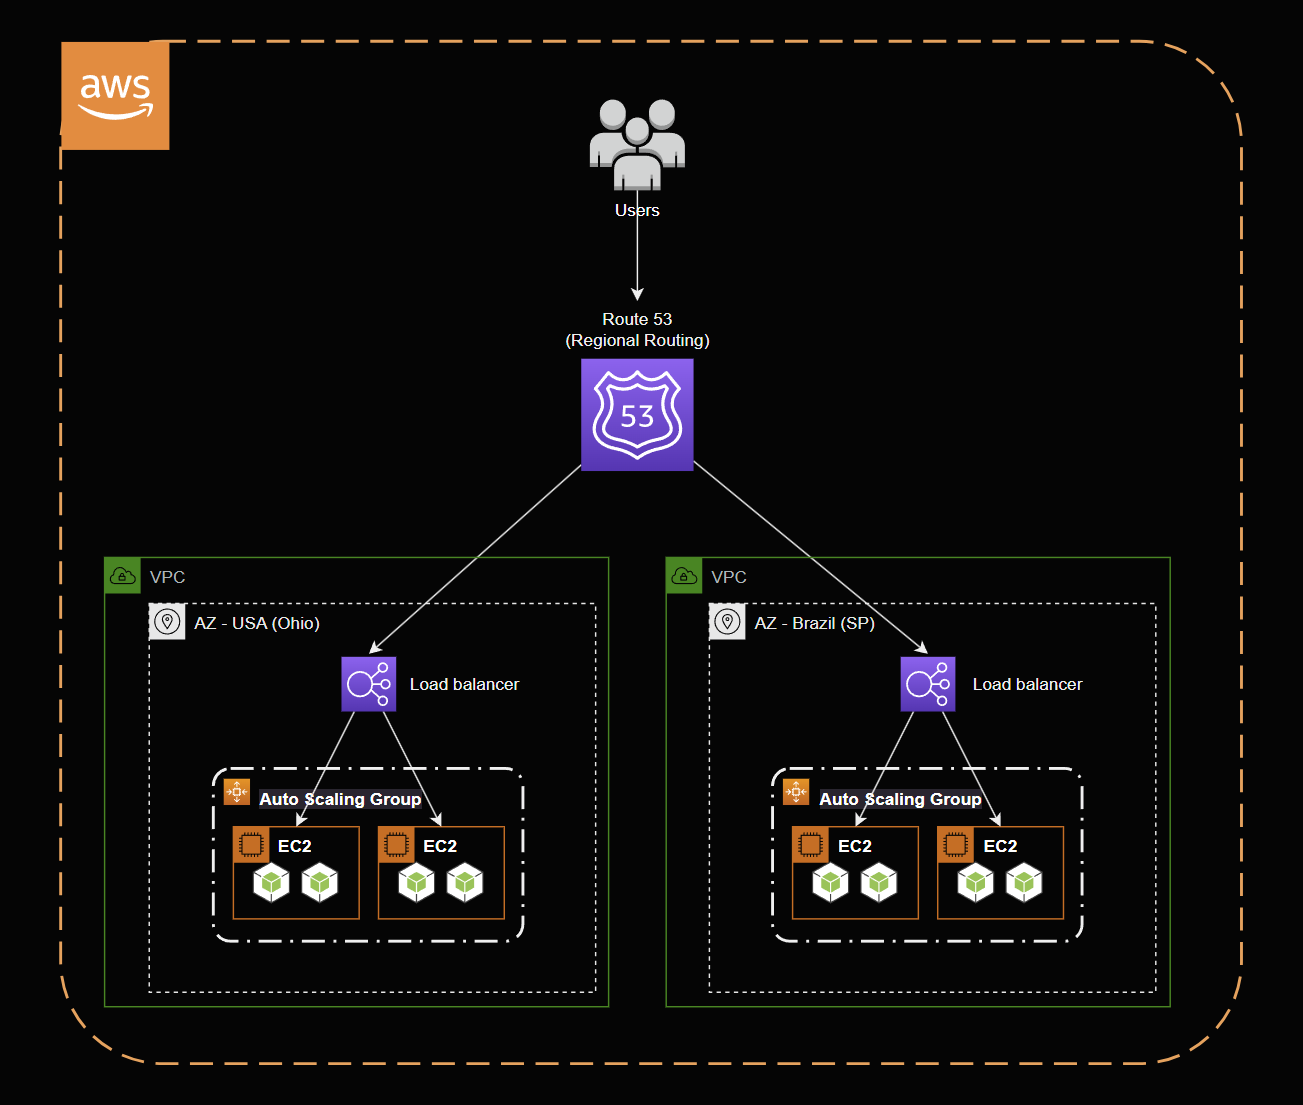
\includegraphics[width=1\textwidth]{drawio/cloud-architecture.png}
\end{figure}

Essas práticas e tecnologias não apenas promovem a alta disponibilidade e desempenho da aplicação, mas também preparam o ambiente para escalar rapidamente em resposta às demandas crescentes, tudo sem intervenção manual, alinhando-se com as melhores práticas de DevOps e com as demandas de uma aplicação moderna. Nas próximas seções, serão apresentados em detalhes as práticas e tecnologias empregadas em cada camada da arquitetura: infraestrutura de computação, balanceamento de carga, escalabilidade, recuperação de falhas, segurança e banco de dados.


\subsection{Planejamento de Infraestrutura}
% Revisado

O planejamento da infraestrutura da plataforma começou com a definição de requisitos e necessidades específicas da aplicação, que incluem:

\begin{itemize}
    \item \textbf{Baixa latência}: Para assegurar uma experiência de usuário fluida e responsiva em tempo real, a plataforma Codeboard precisa operar com baixa latência.
    \item \textbf{Alta disponibilidade}: Codeboard deve estar acessível 24/7, garantindo operação contínua, mesmo durante atualizações e manutenções.
    \item \textbf{Escalabilidade}: A plataforma deve suportar um grande número de usuários simultâneos, aumentando ou diminuindo seus recursos conforme a demanda.
    \item \textbf{Resiliência}: Codeboard precisa de mecanismos de recuperação automática frente a falhas de hardware ou software, sem impacto na experiência do usuário.
    \item \textbf{Custo-efetividade}: A infraestrutura deve ser otimizada para minimizar custos, evitando ociosidade de recursos.
    \item \textbf{Facilidade de gerenciamento}: a infraestrutura deve ser simples de gerenciar, utilizando práticas de DevOps, como \emph{Infra-as-Code} (IaC).
    \item \textbf{Segurança}: A plataforma deve ser protegida contra ameaças e ataques cibernéticos.
    \item \textbf{Monitoramento}: A plataforma deve contar com métricas e logs para acompanhar desempenho e integridade.
\end{itemize}

A hospedagem na Amazon Web Services (AWS) tornou-se uma escolha estratégica devido à sua ampla variedade de serviços, escalabilidade, confiabilidade e presença global de data centers. A infraestrutura global da AWS habilita a arquitetura \emph{Multi-Region Active-Active}, crucial para atender aos requisitos de desempenho e disponibilidade descritos.  Além disso, o \emph{free tier} da AWS foi um diferencial importante, possibilitando o desenvolvimento e os testes iniciais sem custos significativos.

Para atender a esses requisitos, foram escolhidos os seguintes serviços da AWS para compor a infraestrutura da plataforma Codeboard:

\begin{itemize}
    \item \textbf{Amazon Elastic Compute Cloud (EC2)}: Fornece instâncias virtuais escaláveis e seguras para execução da aplicação.
    \item \textbf{Amazon Elastic Load Balancing (ELB)}: Distribui o tráfego entre instâncias EC2, garantindo alta disponibilidade e escalabilidade.
    \item \textbf{AWS Auto Scaling}: Ajusta automaticamente a capacidade das instâncias EC2 conforme a demanda.
    % \item \textbf{Amazon DocumentDB}: serviço de banco de dados NoSQL que fornece instâncias gerenciadas de bancos de dados MongoDB.
    % \item \textbf{Amazon ElastiCache}: serviço de cache em memória que fornece instâncias gerenciadas de Redis.
    \item \textbf{Amazon Virtual Private Cloud (VPC)}: Cria uma rede virtual com sub-redes privadas, gateways de internet e regras de firewall.
    \item \textbf{Amazon Route 53}: Configura registros de DNS, oferece balanceamento de carga entre regiões geográficas e failover.
    \item \textbf{Amazon CloudWatch}: Proporciona métricas, logs e alarmes para monitorar a saúde e o desempenho da aplicação.
    \item \textbf{AWS Identity and Access Management (IAM)}: Gerencia o controle de acesso, permitindo a criação de usuários, grupos e políticas.
    \item \textbf{AWS Certificate Manager (ACM)}: Facilita a criação, renovação e implantação de certificados SSL/TLS para segurança de dados.
\end{itemize}

Essas escolhas de serviço atendem diretamente às necessidades de desempenho, segurança e custo, alinhando a infraestrutura às metas de alta disponibilidade e resiliência exigidas pela plataforma.


\subsection{Implementação de Infraestrutura como Código com Terraform}
% Revisado

Para assegurar um processo de implantação de infraestrutura que seja eficiente, escalável e replicável, a plataforma Codeboard utiliza o \emph{Terraform} como ferramenta de \emph{Infrastructure as Code} (IaC).

A utilização do Terraform como IaC garante que a infraestrutura seja declarativa e executada de forma idempotente, o que significa que recursos existentes não são recriados desnecessariamente a cada execução. Isso resulta em um gerenciamento mais eficiente dos recursos e em um controle de mudanças mais preciso. Foram estabelecidos módulos para tratar de diferentes aspectos da infraestrutura, como rede, segurança e recursos de computação, permitindo que seja possível trabalhar isoladamente em partes distintas da arquitetura sem necessidade de intervenção manual entre essas partes.


\section{Infraestrutura de Computação}

Dada a adoção do modelo \emph{Multi-Region Active-Active}, a infraestrutura de computação da Codeboard foi arquitetada para operar de maneira distribuída através de diferentes regiões geográficas da AWS. Essa abordagem garante, além de uma resposta eficiente a eventuais falhas regionais, uma proximidade maior com os usuários, o que ajuda a reduzir a latência. A infraestrutura de computação integra múltiplos componentes, incluindo instâncias EC2, balanceamento de carga, escalabilidade automática, monitoramento, e diversos mecanismos para segurança e recuperação de falhas, criando um ambiente robusto que sustenta a operação contínua e eficiente da plataforma Codeboard.

\subsection{Servidor Virtual}
% Revisado

Para hospedar a aplicação da plataforma Codeboard, foram escolhidas instâncias EC2 do tipo \emph{t3.micro}, adequadas ao estudo de caso pelos seguintes motivos: 

\begin{itemize}
    \item \textbf{Custo}: As instâncias t3.micro fazem parte do \emph{free tier} da AWS, oferecendo 12 meses de uso gratuito, o que torna essa opção financeiramente viável para a fase inicial do projeto.
    \item \textbf{Desempenho Escalável}: Com capacidade de burst, essas instâncias podem fornecer recursos adicionais de CPU temporariamente, sem custos extras, atendendo a picos de demanda.
    \item \textbf{2 vCPUs}: As instâncias t3.micro possuem 2 vCPUs, que é o mínimo recomendado para a aplicação da plataforma Codeboard, que opera em um \emph{cluster} de processos, onde cada processo é uma aplicação Node.js que é responsável pelo back-end.
    \item \textbf{1 GB de memória RAM}: A memória de 1 GB é adequada para a Codeboard, pois sua função de intermediação de mensagens em tempo real requer um baixo consumo de memória.
    \item \textbf{Armazenamento em disco SSD}: Embora a Codeboard não faça uso intensivo de disco, o armazenamento SSD nas instâncias t3.micro oferece maior velocidade e confiabilidade, beneficiando a estabilidade do sistema.
\end{itemize}

As instâncias EC2 foram configuradas com o sistema operacional \emph{Ubuntu 24.04 LTS}, o servidor web \emph{NGINX}, o gerenciador de processos \emph{PM2} e outras ferramentas para auxiliar no processo de configuração da instância: \emph{Git}, \emph{Node.js}, \emph{NPM}. A escolha do Ubuntu 24.04 LTS deve-se à sua estabilidade e suporte de longo prazo para atualizações de segurança. O NGINX atua como um servidor web reverso, redirecionando o tráfego HTTPS para os processos Node.js que executam a Codeboard. Já o PM2 gerencia esses processos, mantendo-os ativos e reiniciando automaticamente em caso de falhas.

\section{Balanceamento de Carga, Escalabilidade e Recuperação de Falhas}
% Revisado

A arquitetura da plataforma Codeboard foi projetada com uma estratégia de balanceamento de carga, escalabilidade e recuperação de falhas que abrange múltiplos níveis de operação, assegurando alta disponibilidade, baixa latência e resiliência. Esta seção apresenta a abordagem utilizada para distribuir de forma eficiente o tráfego e garantir que a aplicação responda de maneira otimizada, mesmo em cenários de alta demanda ou falhas inesperadas.

O balanceamento de carga entre processos permite uma distribuição uniforme das requisições entre processos individuais da aplicação, garantindo o uso eficiente dos recursos da instância. Para lidar com o tráfego em servidores múltiplos, foi configurado uma segunda camada de balanceamento de carga que distribui as requisições entre instâncias EC2 da AWS, de modo que a aplicação possa escalar horizontalmente conforme a demanda. Para maximizar a disponibilidade global e reduzir a latência para usuários em diferentes localidades, foi implementado um balanceamento de carga geográfico entre regiões da AWS, utilizando o Route 53 para redirecionar o tráfego para a região mais próxima do usuário. 

Mecanismos de recuperação automática de falhas foram configurados em cada nível. Esses mecanismos monitoram continuamente a saúde dos processos e das instâncias, substituindo automaticamente recursos que falhem e garantindo a continuidade da aplicação. Essa estrutura multissetorial de balanceamento e recuperação permite que a plataforma Codeboard mantenha uma operação robusta e confiável, capaz de lidar com flutuações de carga e com interrupções inesperadas.

Nas seções a seguir, serão detalhadas cada uma das três camadas de balanceamento de carga, escalabilidade e recuperação de falhas, demonstrando como esses mecanismos trabalham juntos para garantir a alta disponibilidade e desempenho da aplicação.

\subsection{Balanceamento de Carga entre Processos}
% Revisado

A aplicação Codeboard opera em um \emph{cluster} de processos, o que torna o balanceamento de carga essencial para distribuir o tráfego de entrada de maneira eficiente. Para isso, o PM2 foi configurado no modo cluster, permitindo a criação de múltiplos processos Node.js que compartilham o mesmo \emph{socket} de rede. Dessa forma, o NGINX redireciona o tráfego entre os processos por meio do módulo \emph{proxy\_pass}, que envia as requisições HTTP para o processo Node.js que executa a Codeboard.

O algoritimo de balanceamento de carga utilizado é o \emph{Round Robin}, que distribui o tráfego de entrada de forma alternada entre os processos do cluster, assegurando que cada processo receba uma quantidade igual de solicitações. A Figura \ref{fig:round-robin-load-balancing} ilustra o funcionamento do algoritmo Round Robin, enquanto a Figura \ref{fig:pm2-cluster-mode} mostra o modo cluster do PM2 em ação.

\begin{figure}[H]
    \centering
    \caption{Balanceamento de Carga com Round Robin}
    \label{fig:round-robin-load-balancing}
    \includegraphics[width=1\textwidth]{diagrams/round-robin-load-balancing.png}
\end{figure} 

\begin{figure}[H]
    \centering
    \caption{Modo Cluster do PM2}
    \label{fig:pm2-cluster-mode}
    \includegraphics[width=1\textwidth]{diagrams/pm2-cluster-mode.png}
\end{figure}

O balanceamento de carga entre processos otimiza o uso dos recursos de CPU e memória, distribuindo a carga de trabalho de maneira uniforme entre os vCPUs das instâncias EC2, garantindo um desempenho estável e eficiente.

\subsection{Recuperação Automática de Falhas em Processos}
% Revisado

O balanceamento de carga entre processos também contribui para a alta disponibilidade e confiabilidade da aplicação. Em caso de falha de um dos processos, o tráfego é automaticamente redirecionado para outros, evitando interrupções para os usuários.

Para reforçar a tolerância a falhas e garantir a alta disponibilidade, foram configurados no PM2 mecanismos de monitoramento e recuperação automática. Esse monitoramento verifica continuamente os processos Node.js e, ao detectar uma falha, reinicia o processo comprometido. A Figura \ref{fig:pm2-fault-tolerance} ilustra o funcionamento do monitoramento e recuperação de falhas pelo PM2, garantindo que a aplicação permaneça em funcionamento mesmo diante de falhas pontuais.


\begin{figure}[H]
    \centering
    \caption{Tolerância à Falhas com PM2}
    \label{fig:pm2-fault-tolerance}
    \includegraphics[width=0.8\textwidth]{diagrams/pm2-fault-tolerance.png}
\end{figure}


\subsection{Balanceamento de Carga entre os Servidores}
% Revisado

A infraestrutura de computação da plataforma Codeboard foi projetada para ser distribuída e redundante, assegurando que o tráfego seja balanceado entre várias instâncias EC2 e entre diferentes regiões geográficas. Para essa finalidade, utilizou-se o AWS Elastic Load Balancing (ELB), que distribui o tráfego de entrada de forma equilibrada entre as instâncias, garantindo alta disponibilidade e escalabilidade da aplicação.

Entre os tipos de ELB disponíveis, como o Application Load Balancer (ALB), Network Load Balancer (NLB) e Classic Load Balancer (CLB), escolheu-se o ALB. Esse balanceador de camada 7 permite o roteamento de tráfego com base em critérios específicos, como URL, cabeçalhos HTTP e métodos HTTP. O ALB foi configurado com um certificado SSL para assegurar a segurança do tráfego HTTPS entre clientes e servidores.

O algoritmo de balanceamento de carga adotado foi o \emph{Round Robin}, que distribui o tráfego de forma equitativa entre as instâncias EC2, garantindo uma divisão equilibrada de requisições.


% TODO: Voltar no capítulo 3 para explicar a importância do Health Check? Testar se a conexão com o banco de dados está funcionando, se a aplicação está respondendo, etc.

Para garantir que apenas instâncias saudáveis recebam tráfego, foram configurados \emph{Health Checks} para monitorar a saúde das instâncias EC2. Os Health Checks realizam verificações periódicas em uma rota específica da aplicação Codeboard, permitindo que o ELB detecte se cada instância está respondendo corretamente. Se uma instância não responder adequadamente ao Health Check, o ELB a marca como indisponível e redireciona o tráfego para outras instâncias saudáveis.

Configurou-se o Health Check com um intervalo de 30 segundos e um tempo limite de 5 segundos, o que significa que o ELB realiza uma verificação a cada 30 segundos e aguarda uma resposta dentro de 5 segundos. Após duas falhas consecutivas, a instância é marcada como indisponível e o tráfego é redirecionado para outras instâncias saudáveis. A Figura \ref{fig:elb-health-check} ilustra o funcionamento do Health Check do ELB.

\begin{figure}[H]
    \centering
    \caption{Health Check do ELB}
    \label{fig:elb-health-check}
    \includegraphics[width=0.8\textwidth]{diagrams/elb-health-check.png}
\end{figure}


\subsection{Escalabilidade Horizontal com Auto Scaling}
% Revisado

Para garantir a alta disponibilidade da plataforma Codeboard, a infraestrutura foi projetada para escalar horizontalmente, permitindo que a aplicação aumente ou reduza seus recursos de acordo com a demanda, sem necessidade de intervenção manual. Essa escalabilidade automática foi implementada com o AWS Auto Scaling, que ajusta a quantidade de instâncias EC2 com base na utilização de recursos.

O Auto Scaling utiliza um Auto Scaling Group (ASG) para monitorar a utilização de CPU nas instâncias EC2 e ajustar a quantidade de instâncias conforme uma política de escalabilidade. Definiram-se gatilhos específicos: quando a utilização de CPU ultrapassa um limite predefinido, uma nova instância é adicionada ao grupo, distribuindo melhor a carga. Inversamente, se a utilização de CPU cair abaixo de um limite, o ASG reduz o número de instâncias, otimizando custos. Foi configurado um número mínimo e máximo de instâncias, garantindo um custo controlado e uma capacidade mínima sempre disponível. A Figura \ref{fig:auto-scaling-horizontal-scalability} ilustra essa escalabilidade horizontal com o Auto Scaling.

\begin{figure}[H]
    \centering
    \caption{Escalabilidade Horizontal com Auto Scaling Group}
    \label{fig:auto-scaling-horizontal-scalability}
    \includegraphics[width=1\textwidth]{diagrams/auto-scaling-horizontal-scalability.png}
\end{figure}

Os limites de gatilhos de escalabilidade foram definidos com base em testes e monitoramento da aplicação, estabelecendo 70\% de uso de CPU para adicionar uma nova instância e 30\% para removê-la. Os valores de instâncias mínima e máxima foram configurados entre 1 e 5, podendo ser ajustáveis conforme previsões de tráfego, sazonalidade e eventos especiais.

\subsection{Recuperação Automática de Falhas em Servidores}
% Revisado

O Auto Scaling do AWS também possui um mecanismo de recuperação automática de falhas, que monitora continuamente a saúde das instâncias EC2. Quando uma instância é marcada como indisponível pelo ELB (por falhar em um Health Check), o Auto Scaling substitui automaticamente a instância defeituosa por uma nova, garantindo que a aplicação da plataforma Codeboard permaneça sempre disponível e resiliente a falhas. Essa combinação de Auto Scaling, ELB e PM2 resulta em uma arquitetura altamente disponível, escalável e confiável. A Figura \ref{fig:auto-scaling-fault-tolerance} ilustra o funcionamento da recuperação automática de falhas com o Auto Scaling.

\begin{figure}[H]
    \centering
    \caption{Recuperação Automática de Falhas com Auto Scaling}
    \label{fig:auto-scaling-fault-tolerance}
    \includegraphics[width=1\textwidth]{diagrams/auto-scaling-fault-tolerance.png}
\end{figure}

Durante a inicialização de uma nova instância, o Auto Scaling aplica um \emph{warmup time} de 180 segundos, período necessário para que a instância esteja completamente operacional. Nesse tempo, são realizadas tarefas como configuração da instância, inicialização da aplicação e estabelecimento de conexões com o banco de dados. Durante o warmup time, a instância permanece indisponível para o ELB, e o tráfego é direcionado para outras instâncias saudáveis. Após o término do warmup, a instância é marcada como disponível e começa a receber tráfego. Esse warmup time ajuda a evitar interrupções na aplicação, garantindo que apenas instâncias totalmente preparadas participem da distribuição de carga.


\subsection{Balanceamento de Carga entre Regiões Geográficas}
% Revisado

A infraestrutura da plataforma Codeboard foi projetada para operar em várias regiões geográficas da AWS, permitindo distribuição do tráfego de usuários entre essas regiões para assegurar alta disponibilidade e baixa latência. Essa configuração de várias regiões não só oferece resiliência em caso de falhas regionais (devido a desastres naturais, falhas de hardware, ou manutenção programada), mas também aproxima a aplicação dos usuários, o que reduz a latência e aprimora a experiência de uso.

Para essa distribuição de tráfego entre regiões, foi configurado o Amazon Route 53, o serviço de DNS da AWS que também oferece balanceamento de carga e failover. Um registro de DNS foi criado para a aplicação da plataforma Codeboard no Route 53, o qual direciona o tráfego para o ELB de cada região geográfica. Devido à natureza de comunicação em tempo real da plataforma, o Route 53 foi configurado com balanceamento de carga baseado em latência, de forma que redireciona o tráfego para a região geográfica mais próxima do usuário, garantindo uma experiência rápida e eficiente. 

\begin{figure}[H]
    \centering
    \caption{Balanceamento de Carga Baseado em Latência com Route 53}
    \label{fig:route-53-geographic-load-balancing}
    \includegraphics[width=1\textwidth]{diagrams/route-53-geographic-load-balancing.png}
\end{figure}

A Figura \ref{fig:route-53-geographic-load-balancing} demonstra o funcionamento do balanceamento de carga baseado em latência do Route 53. Quando um usuário faz uma solicitação DNS, o Route 53 primeiro identifica a localização geográfica do usuário com base em seu endereço IP. Em seguida, redireciona o tráfego para a região mais próxima, que consequentemente possui a menor latência, melhorando a experiência do usuário. Esse balanceamento de carga geográfico garante que a plataforma opere de forma eficiente, independentemente da localização dos usuários.

\section{Segurança da Infraestrutura}
% Revisado

A segurança da infraestrutura é um aspecto essencial para garantir a proteção dos dados e a continuidade das operações da plataforma Codeboard. Nesta seção, são discutidas as medidas de segurança implementadas para prevenir acesso não autorizado, proteger o tráfego de dados e garantir a confiabilidade da infraestrutura. Essas práticas abrangem desde o controle de acesso aos recursos de computação até a aplicação de criptografia de dados, assegurando a integridade e a privacidade das informações dos usuários. 

\subsection{Controle de Acesso}
% Revisado

Para proteger a infraestrutura computacional da plataforma Codeboard, várias políticas de segurança foram implementadas, incluindo:

\begin{itemize}
    \item \textbf{AWS Identity and Access Management (IAM)}: políticas e papéis no IAM foram criados para controlar o acesso aos recursos da AWS, aplicando o princípio do menor privilégio. As instâncias EC2, por exemplo, possuem permissões restritas, limitadas apenas às ações necessárias para o funcionamento da aplicação.
    \item \textbf{Firewall}: regras de firewall foram configuradas no \emph{Security Group} da VPC para restringir o tráfego de entrada e saída das instâncias EC2. Somente as portas essenciais para a aplicação estão abertas: a porta 80 (HTTP) é acessível apenas pelo ELB, enquanto a porta 22 (SSH) está disponível exclusivamente para IPs autorizados. Todas as demais portas de entrada são bloqueadas.
    \item \textbf{Chaves SSH}: chaves SSH foram geradas para garantir a autenticação segura de usuários no acesso remoto às instâncias EC2.
\end{itemize}

Além disso, as instâncias EC2 não são acessadas diretamente; o tráfego de entrada passa pelo ELB, que distribui as conexões de forma uniforme. O ELB está configurado com um certificado SSL para garantir a criptografia do tráfego entre cliente e servidor, protegendo os dados em trânsito. Seu Security Group permite apenas o tráfego de entrada na porta 443 (HTTPS).

\subsection{Criptografia de Dados em Trânsito}
% Revisado

Para assegurar a segurança dos dados em trânsito, um certificado SSL foi configurado no ELB para criptografar o tráfego entre o cliente e o servidor. Esse certificado, emitido pelo AWS Certificate Manager (ACM), é gratuito e gerenciado, sendo adequado para serviços da AWS. A configuração inclui um domínio personalizado da plataforma Codeboard, disponível em https://codeboard.pitrol.dev/, o que garante a autenticidade e a integridade das conexões HTTPS. Com isso, a criptografia dos dados em trânsito protege contra interceptações e garante a privacidade e a segurança dos usuários.

% TODO?: \subsection{Rotatividade de Chaves e Segredos}

\section{Banco de Dados MongoDB}
% Revisado

O banco de dados escolhido para a plataforma Codeboard foi o MongoDB, uma solução NoSQL amplamente utilizada por sua flexibilidade, escalabilidade e alto desempenho em aplicações modernas. Diversas abordagens poderiam ser adotadas para hospedar o MongoDB, incluindo instalações locais, máquinas virtuais, contêineres Docker e serviços gerenciados na nuvem. No caso da Codeboard, optou-se pelo \emph{MongoDB Atlas}, um serviço gerenciado pela própria MongoDB que opera sobre infraestruturas robustas como a AWS, Google Cloud Platform e Microsoft Azure.

Essa escolha trouxe diversas vantagens, incluindo alta disponibilidade, escalabilidade e segurança integradas. O MongoDB Atlas proporciona funcionalidades como backups automáticos, monitoramento em tempo real, escalabilidade ajustável e criptografia de dados em trânsito e em repouso, além de integração com outros serviços da AWS. Para atender às necessidades iniciais da aplicação, foi selecionada a instância \emph{M10}, que oferece 2 GB de armazenamento e 0,5 GB de RAM, com suporte a escalabilidade para acomodar futuras demandas.

A adoção do MongoDB Atlas permite que a equipe foque no desenvolvimento da aplicação, enquanto a gestão do banco de dados é simplificada por meio de recursos automatizados, garantindo a robustez e a eficiência no gerenciamento dos dados da plataforma.


\subsection{Escalabilidade Vertical Automática}
% Revisado

O banco de dados MongoDB da plataforma Codeboard foi configurado para escalar verticalmente de maneira automática, garantindo que possa atender ao crescimento das demandas de forma eficiente. A escalabilidade vertical consiste em aumentar os recursos de uma única instância, como CPU, memória e armazenamento, sem a necessidade de configurar múltiplas réplicas ou lidar com a complexidade da escalabilidade horizontal.

A escolha pela escalabilidade vertical, em vez da horizontal, foi fundamentada por duas razões principais:
\begin{enumerate}
    \item \textbf{Custo e Complexidade}: A escalabilidade horizontal envolve a distribuição de dados e cargas de trabalho entre múltiplas instâncias, o que requer configurações avançadas e ferramentas específicas, como sharding. Para um banco de dados com baixa utilização de recursos, a escalabilidade horizontal representaria um custo desnecessário e maior complexidade operacional.
    \item \textbf{Adequação ao Escopo Atual}: O uso inicial da instância M10 do MongoDB Atlas, com 2 GB de armazenamento e 0,5 GB de RAM, provou ser suficiente para as necessidades da aplicação. No entanto, a escalabilidade vertical automática garante que, conforme a demanda cresça, a infraestrutura acompanhe esse crescimento sem interrupções.
\end{enumerate}

O MongoDB Atlas permite configurar a escalabilidade vertical de forma automática, ajustando a capacidade da instância com base na utilização de recursos. Os gatilhos predefinidos monitoram métricas de desempenho, como:
\begin{itemize}
    \item \textbf{CPU}: Se a utilização ultrapassar um limite definido de 75\% na última hora, a capacidade da instância é aumentada automaticamente.
    \item \textbf{Memória}: Um uso persistente acima de uma faixa segura de 90\% por pelo menos 10 minutos dispara o aumento de recursos.
    \item \textbf{Armazenamento}: Quando o espaço disponível atinge um limite crítico de 90\%, a capacidade de armazenamento é ampliada. 
\end{itemize}


Da mesma forma, a escalabilidade vertical também reduz a capacidade da instância quando os recursos são subutilizados, ajudando a otimizar custos operacionais sem sacrificar o desempenho. A Figura \ref{fig:mongodb-atlas-vertical-scalability} ilustra o funcionamento da escalabilidade vertical automática configurada no MongoDB Atlas.

\begin{figure}[H]
    \centering
    \caption{Escalabilidade Vertical Automática no MongoDB Atlas}
    \label{fig:mongodb-atlas-vertical-scalability}
    \includegraphics[width=1\textwidth]{diagrams/mongodb-atlas-vertical-scalability.png}
\end{figure} 

Os benefícios da escalabilidade vertical automática no MongoDB Atlas são diversos e contribuem significativamente para a eficiência operacional da plataforma Codeboard, diminuindo a complexidade, reduzindo custos e automatizando o gerenciamento de recursos do banco de dados. Essa abordagem garante que o banco esteja sempre preparado para atender às demandas crescentes da aplicação, sem a necessidade de interrupções ou intervenções manuais.


\subsection{Backup, Controle de Acesso e Segurança de Dados}
% Revisado

Para atender aos requisitos de segurança e confiabilidade da plataforma Codeboard, foi implementada uma estratégia robusta que abrange tanto o gerenciamento de backups quanto o controle de acesso ao banco de dados e a proteção dos dados em trânsito e em repouso.

Os backups automáticos realizados pelo MongoDB Atlas garantem a preservação e recuperação de dados em caso de falhas ou perdas acidentais, com uma política de retenção que permite a restauração para pontos no tempo ao longo de 14 dias. Adicionalmente, backups sob demanda oferecem flexibilidade para proteger os dados em momentos críticos, como antes de atualizações ou mudanças significativas.

No que diz respeito à segurança, políticas rigorosas de controle de acesso foram implementadas para restringir conexões não autorizadas. Isso inclui o uso de \emph{Whitelists} de IPs e autenticação com credenciais específicas para diferentes níveis de permissão. Além disso, a criptografia de dados, tanto em trânsito quanto em repouso, protege contra interceptações e acessos indevidos, utilizando tecnologias SSL e armazenamento seguro no MongoDB Atlas.

Essas medidas asseguram que os dados da plataforma permaneçam seguros, disponíveis e protegidos contra uma ampla gama de riscos e ameaças.

\section{Banco de dados Redis}
% Revisado

O Redis desempenha um papel crucial na infraestrutura da plataforma Codeboard, servindo como um banco de dados chave-valor em memória de alta performance. Sua velocidade, simplicidade e capacidade de escalabilidade o tornam ideal para atender às necessidades de aplicações que exigem processamento rápido de dados em tempo real, como é o caso da Codeboard. Nesta seção, serão explorados os detalhes de sua configuração, os benefícios de utilizar uma solução gerenciada e as práticas implementadas para garantir a segurança, disponibilidade e desempenho do banco de dados.

\subsection{Provedor de Banco de Dados}
% Revisado

O banco de dados Redis da plataforma Codeboard está hospedado no \emph{Redis Cloud}, uma solução gerenciada pela própria Redis. Essa escolha foi motivada pela robustez e confiabilidade do serviço, que elimina a necessidade de gerenciamento manual da infraestrutura de banco de dados, além de oferecer recursos avançados como monitoramento, backup e suporte técnico especializado.

O Redis Cloud proporciona uma infraestrutura otimizada para alta disponibilidade e desempenho, com suporte a escalabilidade automática para lidar com variações de carga. Além disso, o uso de uma solução gerenciada permite que a equipe foque no desenvolvimento e na operação da aplicação, ao invés de dedicar tempo e recursos ao gerenciamento do banco de dados.

\subsection{Sharding e Replicação}
% Revisado

Para garantir alta disponibilidade e baixa latência, o Redis foi configurado com sharding e replicação. A abordagem de escalabilidade horizontal, baseada no sharding, distribui os dados entre múltiplas réplicas em diferentes nós, permitindo que o banco de dados suporte um grande volume de transações simultâneas sem comprometer o desempenho.

O sharding foi configurado de forma automática pelo Redis Cloud, que gerencia a alocação de dados e o balanceamento de carga entre shards. Já a replicação assegura a resiliência do sistema, criando réplicas secundárias de cada shard. Em caso de falha de um nó, o Redis Cloud promove automaticamente uma réplica para substituí-lo, garantindo continuidade no serviço.

\subsection{Controle de Acesso e Segurança}
% Revisado

A segurança do banco de dados Redis foi configurada com foco em prevenir acessos não autorizados e proteger os dados transmitidos. As políticas de controle de acesso incluem autenticação por senha e restrições baseadas em IP, permitindo conexões apenas de hosts autorizados. Essa abordagem reduz significativamente o risco de acessos externos indevidos.

Para garantir a proteção dos dados em trânsito, o tráfego entre os clientes e o Redis é criptografado utilizando TLS, prevenindo interceptações e acessos maliciosos.

Dado o papel do Redis na plataforma Codeboard, que é utilizado principalmente para dados temporários, não foram configurados backups automáticos. Os dados críticos da aplicação são armazenados no MongoDB, que conta com backups automáticos e políticas de retenção robustas. Essa estratégia assegura que, mesmo em caso de perda de dados no Redis, eles possam ser facilmente regenerados sem impacto significativo na operação.


\section{Distribuição de Conteúdo (CDN)}
% Revisado

Uma \emph{Content Delivery Network} (CDN) é uma rede de servidores distribuídos geograficamente que trabalham em conjunto para entregar conteúdos da web com rapidez e eficiência. Ao armazenar cópias dos arquivos em locais próximos aos usuários finais, uma CDN reduz o tempo de carregamento, diminui a carga no servidor de origem e melhora a experiência do usuário.

\subsection{Plataforma de CDN}
% Revisado

A utilização de uma CDN desempenha um papel essencial na entrega rápida e eficiente do front-end da plataforma Codeboard. A infraestrutura foi implementada utilizando a plataforma \emph{Vercel}, que combina os benefícios de uma CDN global com recursos de plataforma como serviço (PaaS), otimizando a experiência dos usuários finais.

O uso da CDN integrada ao Vercel traz diversos benefícios, incluindo:

\begin{itemize}
    \item Redução de latência: Ao distribuir o conteúdo para servidores localizados próximos aos usuários, o tempo de resposta é minimizado.
    \item Alta disponibilidade: A CDN utiliza redundância para garantir que os conteúdos estejam sempre acessíveis, mesmo em caso de falhas em servidores específicos.
    \item Escalabilidade automática: A infraestrutura da CDN lida automaticamente com picos de tráfego, assegurando desempenho consistente.
    \item Segurança aprimorada: Recursos como mitigação de DDoS e controle de acesso a nível de borda ajudam a proteger a plataforma contra ataques.
\end{itemize}

\subsection{Configuração da CDN}
% Revisado

No contexto da Codeboard, a configuração da CDN foi simplificada pela utilização do Vercel. A plataforma automaticamente gerencia o cache de conteúdo estático e implementa o cache dinâmico conforme necessário, baseado nos cabeçalhos de resposta configurados na aplicação. Regras de invalidade de cache são aplicadas automaticamente durante os deploys, garantindo que os usuários sempre acessem a versão mais recente da aplicação.

Além disso, a CDN do Vercel está totalmente integrada com o sistema de build e deploy contínuos, sincronizando alterações no front-end com a rede de distribuição em tempo real. Essa abordagem garante alta performance e agilidade no lançamento de novas funcionalidades.


\section{Monitoramento}
% Revisado

% Por que monitoramento é importante? R: Garantir a disponibilidade, desempenho e segurança da aplicação, atuando proativamente para evitar falhas e interrupções.

O monitoramento é um elemento crítico para garantir a disponibilidade, o desempenho e a segurança da aplicação. Por meio do acompanhamento contínuo de métricas e logs, é possível identificar e mitigar problemas proativamente, antes que causem interrupções ou degradação no serviço. Esta seção detalha como o monitoramento é implementado na plataforma Codeboard, abrangendo tanto a aplicação quanto os recursos de infraestrutura em nuvem.

\subsection{Monitoramento da Aplicação}
% Revisado

% Como o monitoramento da aplicação é feito? R: CloudWatch
% Quais métricas são monitoradas? R: Requisições, logs de erros, etc.

O monitoramento da aplicação é realizado utilizando o \emph{Amazon CloudWatch}, um serviço nativo da AWS que permite coletar, analisar e agir com base em dados e logs de desempenho. As métricas monitoradas incluem:

\begin{itemize}
    \item \textbf{Requisições}: Número de requisições recebidas, permitindo analisar padrões de tráfego e identificar possíveis gargalos.
    \item \textbf{Logs de erros}: Registro de falhas e exceções capturados em tempo real, possibilitando a identificação de problemas no código ou na infraestrutura.
    \item \textbf{Latência}: Tempo médio de resposta das requisições, monitorando a eficiência da aplicação e identificando possíveis pontos de melhoria.
\end{itemize}

Os dados coletados são apresentados em dashboards personalizados, oferecendo uma visão consolidada da saúde da aplicação e facilitando a identificação de padrões anormais.


\subsection{Monitoramento de Recursos da Nuvem}
% Revisado

% Como o monitoramento de recursos da nuvem é feito? R: CloudWatch
% Quais métricas são monitoradas? R: CPU, memória, etc.

Além da aplicação, os recursos da infraestrutura de computação em nuvem também são monitorados por meio do Amazon CloudWatch. Essa abordagem assegura que os componentes subjacentes, como os servidores, operem dentro dos parâmetros esperados.

As principais métricas monitoradas incluem:

\begin{itemize}
    \item \textbf{Uso de CPU}: Percentual de utilização do processador, indicando se os recursos estão sendo subutilizados ou sobrecarregados.
    \item \textbf{Uso de memória}: Quantidade de memória consumida, essencial para evitar problemas de desempenho devido à falta de recursos.
    \item \textbf{Tamanho de disco}: Utilização de armazenamento, permitindo antecipar a necessidade de expansão.
\end{itemize}

O monitoramento desses recursos é fundamental para identificar gargalos de desempenho e escalonar a infraestrutura de maneira eficiente.

\subsection{Alertas e Notificações}
% Revisado

O sistema de monitoramento da plataforma Codeboard conta com uma estratégia robusta de alertas para garantir respostas rápidas a possíveis incidentes. Os alertas são configurados no Amazon CloudWatch, permitindo a detecção e notificação de anomalias em tempo real.

As principais características do sistema de alertas incluem critérios personalizáveis, permitindo a configuração de limites para métricas específicas, como latência acima de 500ms, uso de CPU superior a 80\% ou erros 5xx que excedam um determinado volume. Além disso, há integração com ferramentas de comunicação, com notificações automáticas enviadas para canais como Slack e e-mail, garantindo que os responsáveis sejam informados imediatamente.

Com essa abordagem, o sistema de alertas fortalece a capacidade da plataforma de reagir rapidamente a eventos adversos, reduzindo o impacto nos usuários e assegurando a continuidade do serviço.